\let\negmedspace\undefined
\let\negthickspace\undefined
\documentclass[journal]{IEEEtran}
\usepackage[a5paper, margin=10mm, onecolumn]{geometry}
%\usepackage{lmodern} % Ensure lmodern is loaded for pdflatex
\usepackage{tfrupee} % Include tfrupee package

\setlength{\headheight}{1cm} % Set the height of the header box
\setlength{\headsep}{0mm}     % Set the distance between the header box and the top of the text

\usepackage{gvv-book}
\usepackage{gvv}
\usepackage{cite}
\usepackage{amsmath,amssymb,amsfonts,amsthm}
\usepackage{algorithmic}
\usepackage{graphicx}
\usepackage{textcomp}
\usepackage{xcolor}
\usepackage{txfonts}
\usepackage{listings}
\usepackage{enumitem}
\usepackage{mathtools}
\usepackage{gensymb}
\usepackage{comment}
\usepackage[breaklinks=true]{hyperref}
\usepackage{tkz-euclide} 
\usepackage{listings}
% \usepackage{gvv}                                        
\def\inputGnumericTable{}                                 
\usepackage[latin1]{inputenc}                                
\usepackage{color}                                            
\usepackage{array}                                            
\usepackage{longtable}                                       
\usepackage{calc}                                             
\usepackage{multirow}                                         
\usepackage{hhline}                                           
\usepackage{ifthen}                                           
\usepackage{lscape}
\begin{document}

\bibliographystyle{IEEEtran}
\vspace{3cm}

\title{9.5.6}
\author{EE24BTECH11018 - Durgi Swaraj Sharma}

% \maketitle
% \newpage
% \bigskip
{\let\newpage\relax\maketitle}

\renewcommand{\thefigure}{\theenumi}
\renewcommand{\thetable}{\theenumi}
\setlength{\intextsep}{10pt} % Space between text and floats


\numberwithin{equation}{enumi}
\numberwithin{figure}{enumi}
\renewcommand{\thetable}{\theenumi}


\textbf{Question:}\\
Find the area of the region lying above the $X$ axis and included between the circle $x^2+y^2=8x$ and inside of the parabola $y^2=4x$. \hfill \brak{12, 2018}
\begin{table}[h!] 
  \centering
  \begin{center}
    \begin{tabular}{|c|c|c|} 
        \hline
            \textbf{Point} & \textbf{Description} & \textbf{Coordinates} \\ 
        \hline
            $A$   & One end of the line segment & $A =$ \myvec{-2 \\ 0} \\ 
        \hline
            $B$   & Other end of line segment & $B =$ \myvec{0 \\ 8}\\ 
        \hline
	    $P$   & Point trisecting the line segment and closer to point \textbf{A} & $P  =$ \myvec{x_1 \\ y_1}\\ 
        \hline
	    $Q$   & The other point trisecting the line segment & $Q  =$ \myvec{x_2 \\ y_2}\\ 
	    \hline
    \end{tabular}
\end{center}  

  \caption{Variables Used}
  \label{tab9-5.6-1}
\end{table}\\
\solution\\
Equation of a circle is of form $\vec{x}^{\top}\vec{V}\vec{x}+2\vec{u}^{\top}\vec{x}+f=0$ with
\begin{align}
	\vec{u}=\myvec{-4\\0}\\
	f=\norm{\vec{u}}^2-r^2\\
	\vec{V}=\myvec{1&0\\0&1}
\end{align}
Equation of parabola with directrix $\vec{n}^{\top}\vec{x}=c$ is given by,
\begin{align}
	g\brak{\vec{x}}=\vec{x}^{\top}\vec{V}\vec{x}+2\vec{u}^{\top}\vec{x}+f=0\\
	\vec{V}=\norm{\vec{n}}^2\vec{I}-e^2\vec{n}\vec{n}^{\top}\\
	\vec{u}=ce^2\vec{n}-\norm{\vec{n}}^2\vec{F}\\
	f=\norm{\vec{n}}^2\norm{\vec{F}}^2-c^2e^2
\end{align}
and for the parabola $y^2=4x$, equation of directrix is, $\myvec{-1&0}\vec{x}=1$
\begin{align}
	\vec{V}&=\myvec{0&0\\0&1}\\
	\vec{u}&=\myvec{-2\\0}\\
	f&=0
\end{align}
The intersection of two conics with parameters $\vec{V}_i,\vec{u}_i,f_i, i=1,2$ is defined as,
\begin{align}
	\vec{x}^{\top}\brak{\vec{V}_1-\vec{V}_2}\vec{x}+2\brak{\vec{u}_1-\vec{u_2}}^{\top}\vec{x}+\brak{f_1-f_2}=0
\end{align} 
On solving we get the points of intersection to be $\myvec{0\\0},\myvec{4\\4}.$\\
Area between the two curves above $X$ axis is,
\begin{align}
	&\int_0^4 2\sqrt{x} dx- \int_0^4 \sqrt{x^2-8x} dx = \frac{12\pi-32}{3} = 1.899 approx.
\end{align}
The area between the curves $y^2=4x, x^2+y^2=8x$ above the $X$ axis is around 1.899 units
\begin{figure}[h!]
   \centering
   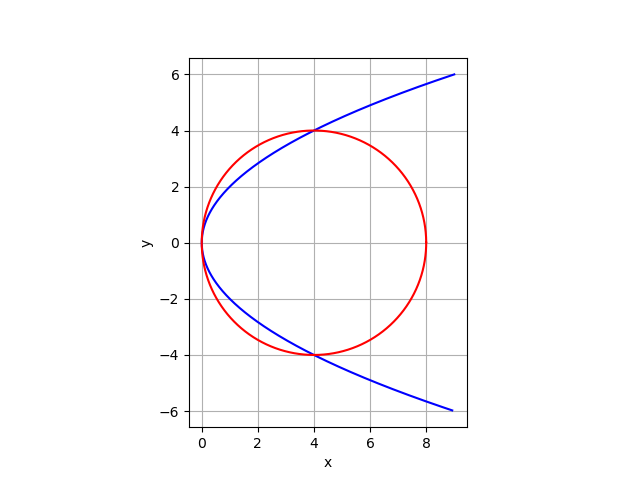
\includegraphics[width = 1\linewidth]{figs/fig.png}
   \caption{Required parabola and circle}
   \label{stemplot}
\end{figure}
\end{document}
